\chapter{Related Work}
\label{chapter:related.work}

This chapter provides an overview of concepts related to this thesis. We
discuss relevant algorithms in brief and talk about similar projects. In the 
first section we discuss the Paxos family of algorithms and projects in 
this domain in the later sections.

\section{Paxos}

Paxos is regarded as the simplest and most obvious of distributed algorithms 
\citep{Lamport01}. It is a consensus protocol used for replication of state
machines in an asynchronous environment \citep{Lamport98}.

A consensus algorithm tries to get a group of processes to agree on a value 
while satisfying its safety requirements%
\sidenote{
  Safety requirements of a consensus algorithm \citep{LamportM04}:
  \begin{inparaenum}[(i)]
    \item \emph{Nontriviality}: A value has to be proposed to be choosen.
    \item \emph{Consistency}: Only one value may be choosen.
    \item \emph{Conservatism}: Only choosen values can be learned.
  \end{inparaenum}
}. 
These processes in the Paxos algorithm can be classified based on their roles
without affecting its correctness:

\begin{itemize}
  \item \emph{Proposer}: A process that can propose values to the group. 
  \item \emph{Acceptor}: Acceptors form the ``memory'' of the algorithm to 
    allow choosing a single value.
  \item \emph{Learner}: The choosen values are ``learned'' by the other 
    processes.
\end{itemize}

\begin{figure}
  \captionstyle{\raggedright}
  \begin{whole}
    \begin{minipage}[t]{\wholewidth}
      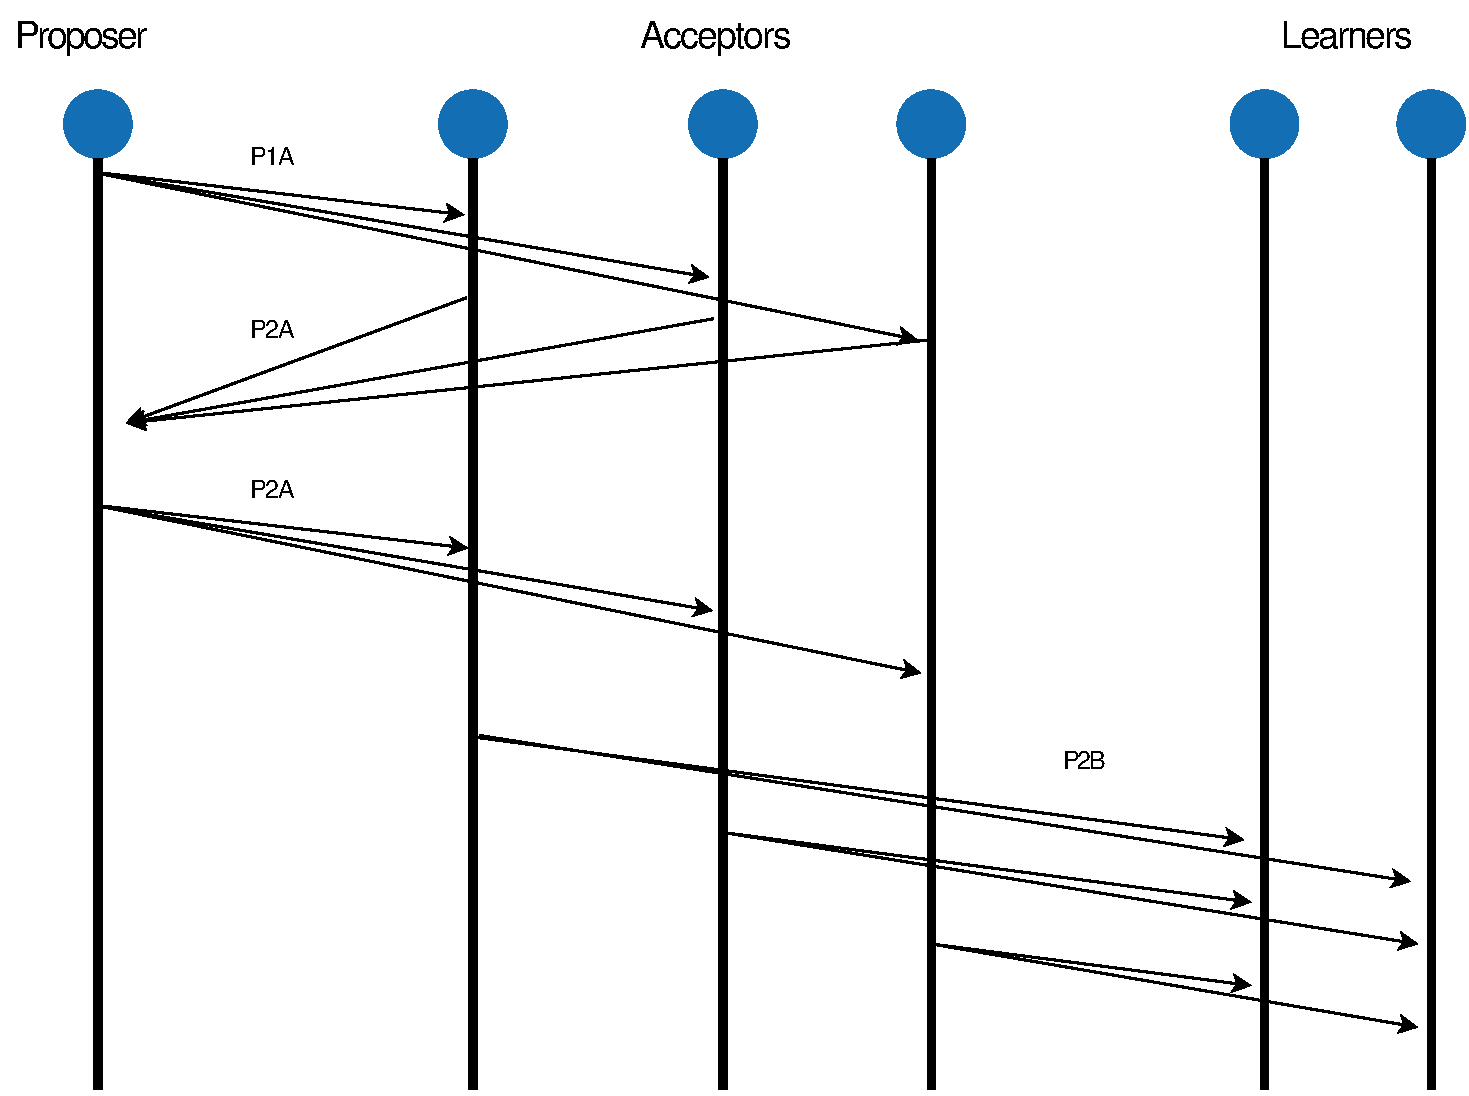
\includegraphics[width=\textwidth]{basic_paxos}
      \caption[Basic Paxos]{%
        Basic Paxos Algorithm: Processes with roles - Proposer, Acceptor, Leader
        - send messages to each other illustrating the flow of the algorithm in
        a failure free instance.}
      \label{figure:basic_paxos}
    \end{minipage}
  \end{whole}
  \normalcaption
\end{figure}

The algorithm proceeds in two phases with each phase having two sub phases.

\begin{itemize}
  \iterm{Phase 1 a}: Proposer select a number \emph{n} and sends it as a
  \emph{prepare} (P1A) message to all the acceptors.
  \iterm{Phase 1 b}: Acceptors compares the \emph{prepare} \emph{n} it receives
  and if it is greater than all previous numbers received as a part of 
  \emph{prepare}, it replies (P1B) with a promise not to accept any number lower
  than \emph{n}.
  \iterm{Phase 2 a}: If the proposer receives a response to its \emph{prepare}
  messages from a quorum%
  \sidenote{
    \emph{Quorum}: Majority agreement of processes.
  }
  , it sends a reply (P2A) back to each of the acceptor with an \emph{accept} 
  message. The message also consists of the value \emph{v} which is the highest 
  numbered proposal among all the responses from the acceptors. In case it is 
  empty, the proposer is free to choose the value.
  \iterm{Phase 2 b}: If the acceptor has not received any \emph{prepare} request
  with a larger number when it receives an \emph{accept} request from the 
  proposer, it sends a message (P2B) to the learner with the accepted value 
  \emph{v}.
  \iterm{Learner}: If the learner receives a message from quorum of acceotor, it
  concludes that the value \emph{v} was choosen.
\end{itemize}  

\subsection{Basic Paxos}

\subsection{Multi-Paxos}

this + paxos made moderately complex

\subsection{Fast Paxos}

\subsection{Cheap Paxos}

\subsection{Ring Paxos}

\subsection{Stoppable Paxos}

This + reconfigurable state machine

\subsection{Other}

Paxos for system builders

Erlang implementations

* gen\_paxos
* ePaxos
* gen\_leader

\section{Google chubby locks}

describe chubby locks

paxos made liveA

\section{Google megastore}

\section{Doozerd}

\section{Zookeeper}

this + ZAB

\section{Riak}

\section{Amazon Dynamo}

\section{Dynamo DB}

\section{Scalaris}

